\documentclass{report}

\usepackage{hyperref}

\usepackage{epstopdf}
\usepackage{amsmath}
\usepackage{amssymb}
\usepackage{subfig}
%\usepackage{multirow}
\usepackage[utf8]{inputenc}
\usepackage[T1]{fontenc}
\usepackage{standalone}
\usepackage{tikz}
\usepackage{tabularx}
\usepackage{float}
\usepackage[section]{placeins}
\usepackage{sverb}
\usepackage{import}
\usepackage{verbatim}
\usepackage{listings}
\usepackage{xcolor}


\graphicspath{{img/}}
\DeclareGraphicsExtensions{.pdf,.png,.jpg,.svg} %For pdflatex



\begin{document}

\begin{titlepage}
    \begin{center}
        \Huge
        \textbf{Przetwarzanie Obrazów Cyfrowych}
        \\ \vspace{1.5cm}
        \Large
        \textbf{Raport z ćwiczenia 2}        
    \end{center}
    \vspace{4.0cm}
    \Large
    Autor: \\
    Dawid Kania    
\end{titlepage}


\section*{
    Obliczanie liczby barw w obrazie
}
\subsection*{
    Obliczanie liczby barw w obrazie RGB
}


\newcommand{\ww}{0.45} %zmienna używana jako parametr opisujące szerokość obrazu zdefiniowana poraz pierwszy w dokumencie
\begin{figure}[H]
    \captionsetup[subfloat]{justification=raggedright,singlelinecheck=false, position=bottom,labelformat=empty} %
    \subfloat[----!matlab/zad1_count.txt:1!----]{\includegraphics[width=\ww\linewidth]{../obrazy/05\_512x512.png }} \hfill%	
    \subfloat[----!matlab/zad1_count.txt:2!----]{\includegraphics[width=\ww\linewidth]{../obrazy/baboon\_512x512.png  }} \hfill% wypełnenie
    \caption{tekst to zmiany} 
    \label{fig:porownanie1} %label który można wykorzystać w tekście za pomocą polecenia \ref{fig:porownanie1}
\end{figure}


\begin{figure}[H]
    \captionsetup[subfloat]{justification=raggedright,singlelinecheck=false, position=bottom,labelformat=empty} %
    \subfloat[----!matlab/zad1_count.txt:3!----]{\includegraphics[width=\ww\linewidth]{../obrazy/lena\_512x512.png     }} \hfill%	
    \subfloat[----!matlab/zad1_count.txt:4!----]{\includegraphics[width=\ww\linewidth]{../obrazy/peppers3\_512x512.png }} \hfill% wypełnenie
    \caption{tekst to zmiany} 
    \label{fig:porownanie1} %label który można wykorzystać w tekście za pomocą polecenia \ref{fig:porownanie1}
\end{figure}





\subsection*{
    Obliczanie liczby barw w obrazie HSV
}


\section*{
    Kwantyzacja obrazów
}

\subsection*{
    Kwantyzacja RGB
}

\renewcommand{\ww}{0.19} 
\begin{figure}[H]
    \captionsetup[subfloat]{justification=raggedright,singlelinecheck=false, position=bottom,labelformat=empty} %
    \subfloat[----!zad2/rgb1/data:1!----]{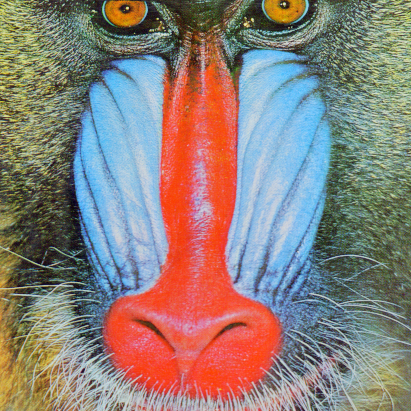
\includegraphics[width=\ww\linewidth]{../zad2/rgb1/I1_ori.png }} \hfill%	
    \subfloat[----!zad2/rgb1/data:2!----]{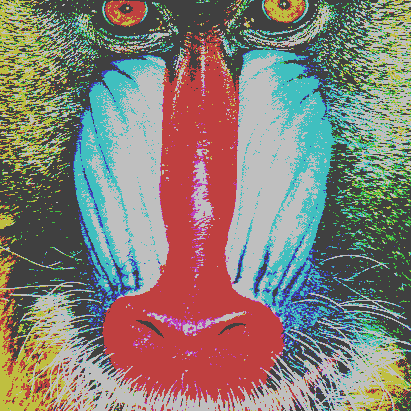
\includegraphics[width=\ww\linewidth]{../zad2/rgb1/I1_222.png }} \hfill%	
    \subfloat[----!zad2/rgb1/data:3!----]{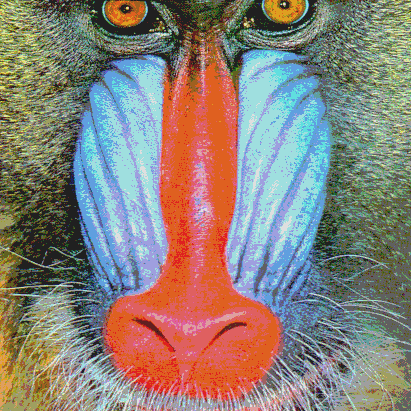
\includegraphics[width=\ww\linewidth]{../zad2/rgb1/I1_444.png }} \hfill% wypełnenie
    \subfloat[----!zad2/rgb1/data:4!----]{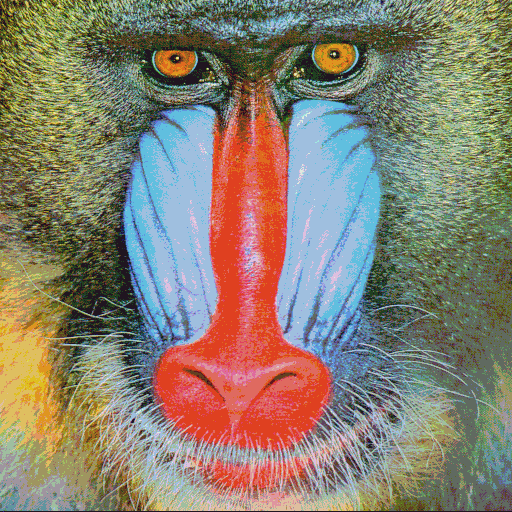
\includegraphics[width=\ww\linewidth]{../zad2/rgb1/I1_464.png }} \hfill%	
    \subfloat[----!zad2/rgb1/data:5!----]{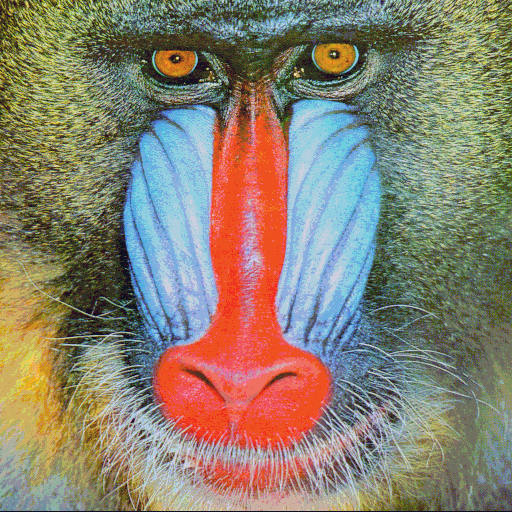
\includegraphics[width=\ww\linewidth]{../zad2/rgb1/I1_884.png }} \hfill% wypełnenie
    \caption{tekst to zmiany} 
    \label{fig:porownanie1} %label który można wykorzystać w tekście za pomocą polecenia \ref{fig:porownanie1}
\end{figure}

\renewcommand{\ww}{0.19} 
\begin{figure}[H]
    \captionsetup[subfloat]{justification=raggedright,singlelinecheck=false, position=bottom,labelformat=empty} %
    \subfloat[----!zad2/rgb2/data:1!----]{\includegraphics[width=\ww\linewidth]{../zad2/rgb2/I1_ori.png }} \hfill%	
    \subfloat[----!zad2/rgb2/data:2!----]{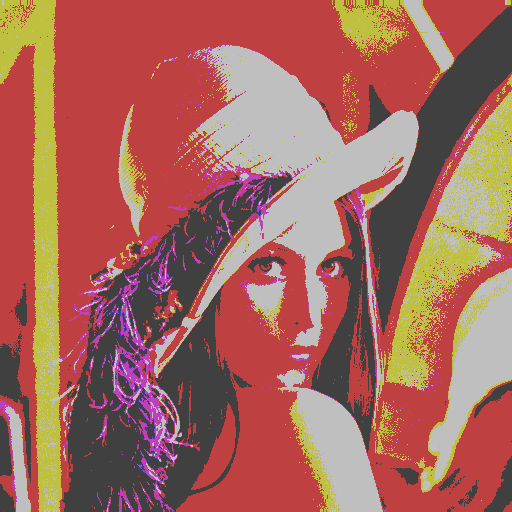
\includegraphics[width=\ww\linewidth]{../zad2/rgb2/I1_222.png }} \hfill%	
    \subfloat[----!zad2/rgb2/data:3!----]{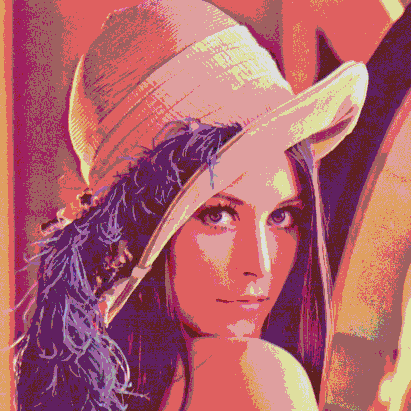
\includegraphics[width=\ww\linewidth]{../zad2/rgb2/I1_444.png }} \hfill% wypełnenie
    \subfloat[----!zad2/rgb2/data:4!----]{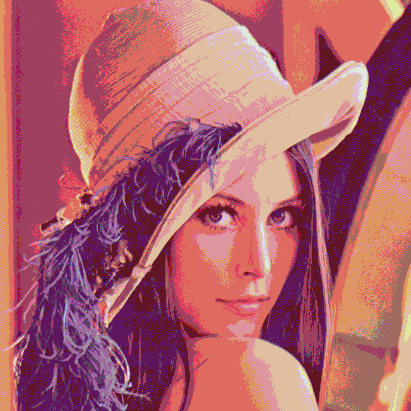
\includegraphics[width=\ww\linewidth]{../zad2/rgb2/I1_464.png }} \hfill%	
    \subfloat[----!zad2/rgb2/data:5!----]{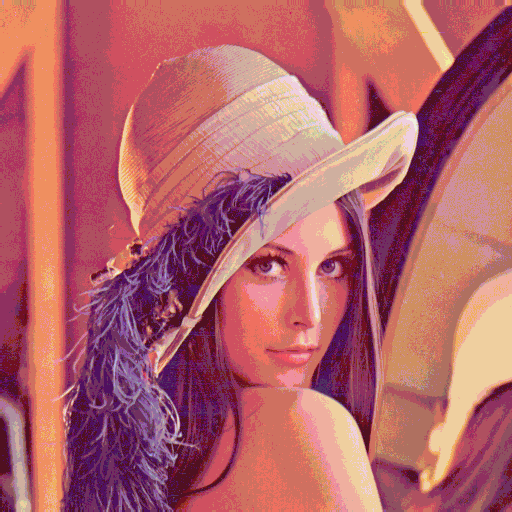
\includegraphics[width=\ww\linewidth]{../zad2/rgb2/I1_884.png }} \hfill% wypełnenie
    \caption{tekst to zmiany} 
    \label{fig:porownanie1} %label który można wykorzystać w tekście za pomocą polecenia \ref{fig:porownanie1}
\end{figure}

\renewcommand{\ww}{0.19} 
\begin{figure}[H]
    \captionsetup[subfloat]{justification=raggedright,singlelinecheck=false, position=bottom,labelformat=empty} %
    \subfloat[----!zad2/rgb3/data:1!----]{\includegraphics[width=\ww\linewidth]{../zad2/rgb3/I1_ori.png }} \hfill%	
    \subfloat[----!zad2/rgb3/data:2!----]{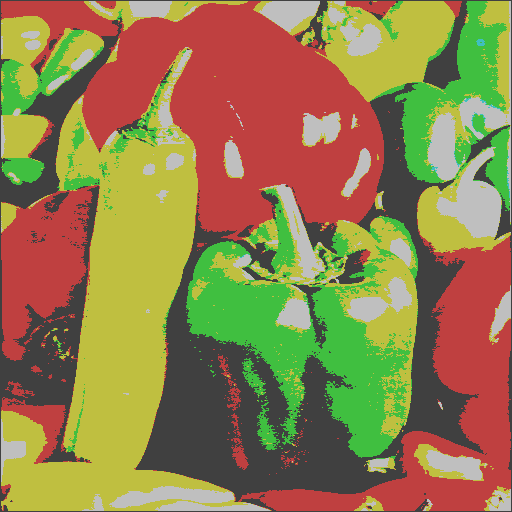
\includegraphics[width=\ww\linewidth]{../zad2/rgb3/I1_222.png }} \hfill%	
    \subfloat[----!zad2/rgb3/data:3!----]{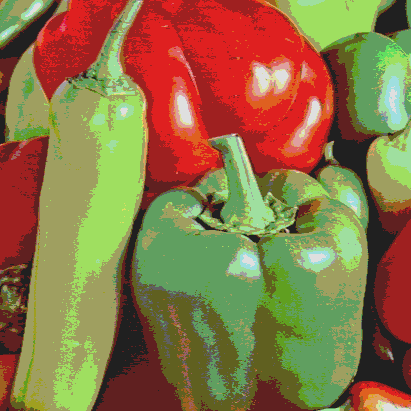
\includegraphics[width=\ww\linewidth]{../zad2/rgb3/I1_444.png }} \hfill% wypełnenie
    \subfloat[----!zad2/rgb3/data:4!----]{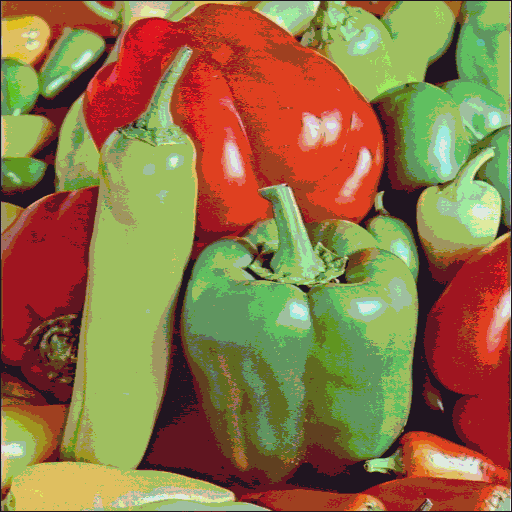
\includegraphics[width=\ww\linewidth]{../zad2/rgb3/I1_464.png }} \hfill%	
    \subfloat[----!zad2/rgb3/data:5!----]{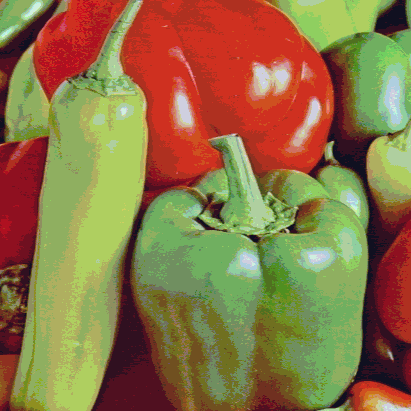
\includegraphics[width=\ww\linewidth]{../zad2/rgb3/I1_884.png }} \hfill% wypełnenie
    \caption{tekst to zmiany} 
    \label{fig:porownanie1} %label który można wykorzystać w tekście za pomocą polecenia \ref{fig:porownanie1}
\end{figure}

\renewcommand{\ww}{0.19} 
\begin{figure}[H]
    \captionsetup[subfloat]{justification=raggedright,singlelinecheck=false, position=bottom,labelformat=empty} %
    \subfloat[----!zad2/rgb4/data:1!----]{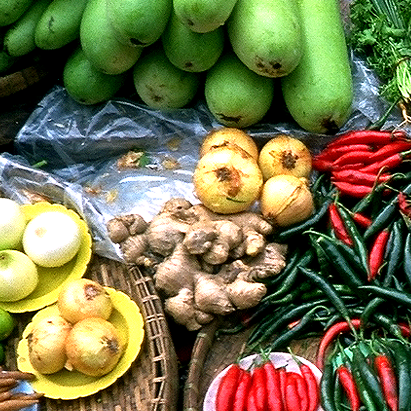
\includegraphics[width=\ww\linewidth]{../zad2/rgb4/I1_ori.png }} \hfill%	
    \subfloat[----!zad2/rgb4/data:2!----]{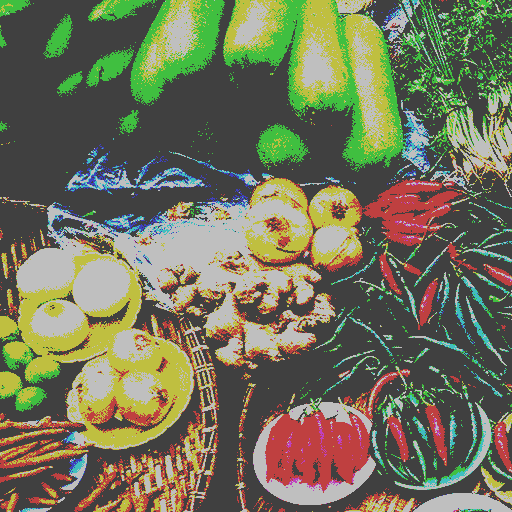
\includegraphics[width=\ww\linewidth]{../zad2/rgb4/I1_222.png }} \hfill%	
    \subfloat[----!zad2/rgb4/data:3!----]{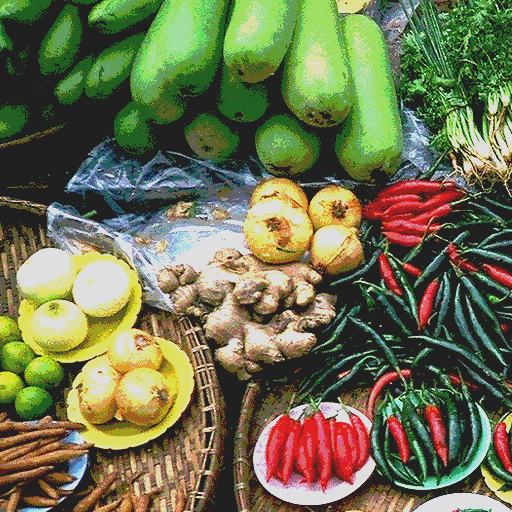
\includegraphics[width=\ww\linewidth]{../zad2/rgb4/I1_444.png }} \hfill% wypełnenie
    \subfloat[----!zad2/rgb4/data:4!----]{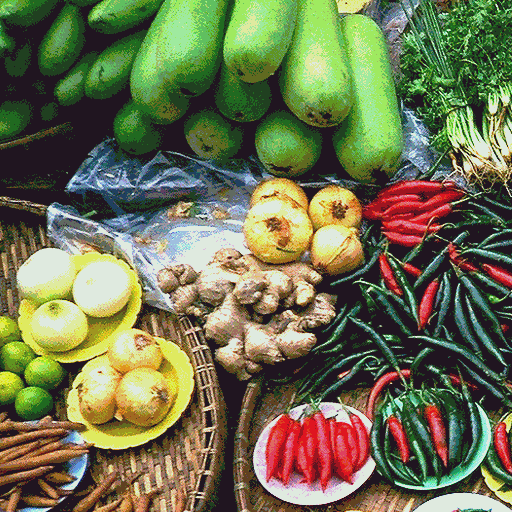
\includegraphics[width=\ww\linewidth]{../zad2/rgb4/I1_464.png }} \hfill%	
    \subfloat[----!zad2/rgb4/data:5!----]{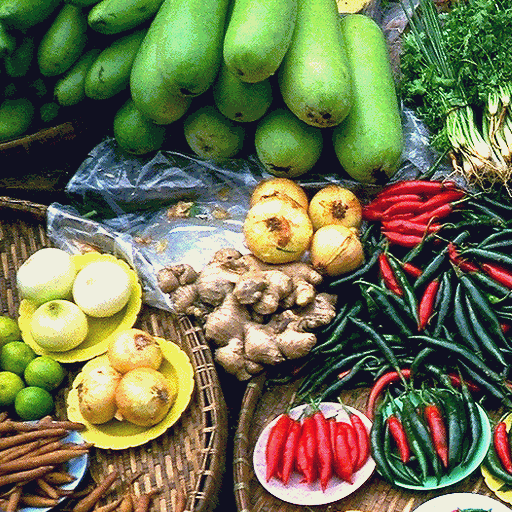
\includegraphics[width=\ww\linewidth]{../zad2/rgb4/I1_884.png }} \hfill% wypełnenie
    \caption{tekst to zmiany} 
    \label{fig:porownanie1} %label który można wykorzystać w tekście za pomocą polecenia \ref{fig:porownanie1}
\end{figure}

\renewcommand{\ww}{0.19} 
\begin{figure}[H]
    \captionsetup[subfloat]{justification=raggedright,singlelinecheck=false, position=bottom,labelformat=empty} %
    \subfloat[----!zad2/rgb5/data:1!----]{\includegraphics[width=\ww\linewidth]{../zad2/rgb5/I1_ori.png }} \hfill%	
    \subfloat[----!zad2/rgb5/data:2!----]{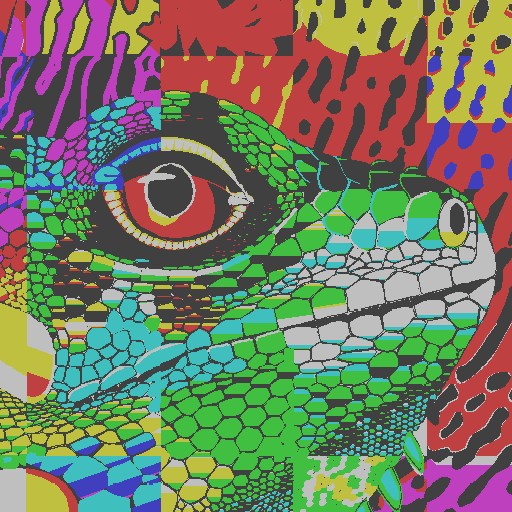
\includegraphics[width=\ww\linewidth]{../zad2/rgb5/I1_222.png }} \hfill%	
    \subfloat[----!zad2/rgb5/data:3!----]{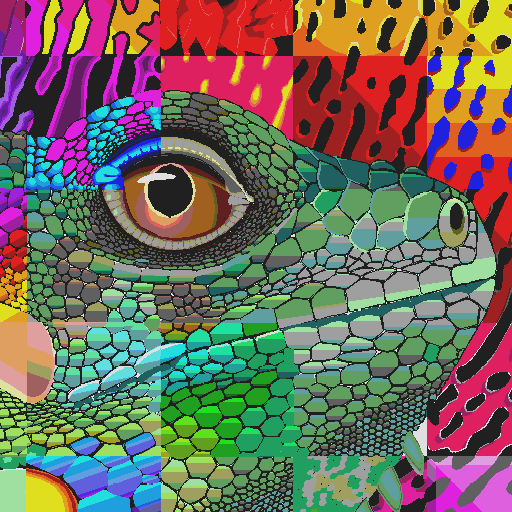
\includegraphics[width=\ww\linewidth]{../zad2/rgb5/I1_444.png }} \hfill% wypełnenie
    \subfloat[----!zad2/rgb5/data:4!----]{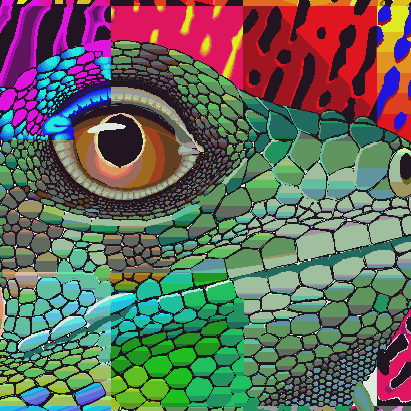
\includegraphics[width=\ww\linewidth]{../zad2/rgb5/I1_464.png }} \hfill%	
    \subfloat[----!zad2/rgb5/data:5!----]{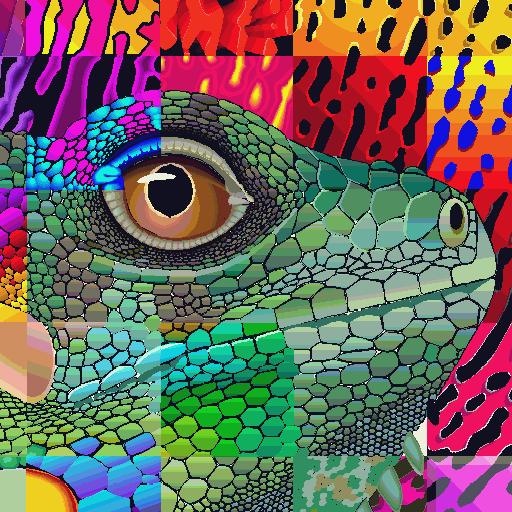
\includegraphics[width=\ww\linewidth]{../zad2/rgb5/I1_884.png }} \hfill% wypełnenie
    \caption{tekst to zmiany} 
    \label{fig:porownanie1} %label który można wykorzystać w tekście za pomocą polecenia \ref{fig:porownanie1}
\end{figure}


\subsection*{
    Kwantyzacja HSV
}

\renewcommand{\ww}{0.30} 
\begin{figure}[H]
    \captionsetup[subfloat]{justification=raggedright,singlelinecheck=false, position=bottom,labelformat=empty} %
    \subfloat[----!zad2/hsv1/data:1!----]{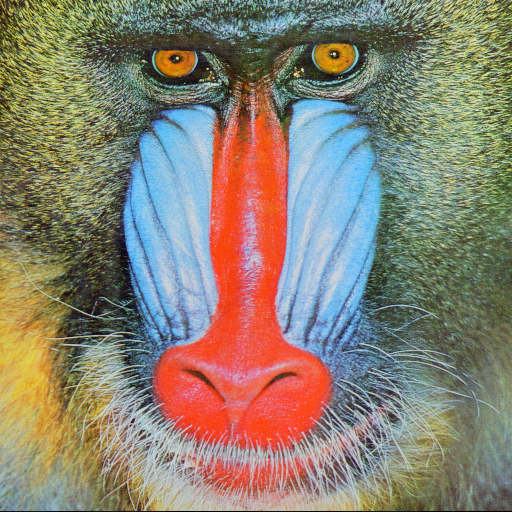
\includegraphics[width=\ww\linewidth]{../zad2/hsv1/I1_ori.png }} \hfill%	
    \subfloat[----!zad2/hsv1/data:2!----]{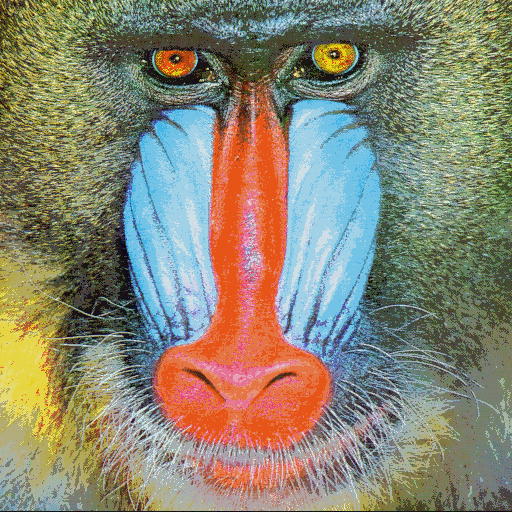
\includegraphics[width=\ww\linewidth]{../zad2/hsv1/I1_222.png }} \hfill%
    \subfloat[----!zad2/hsv1/data:3!----]{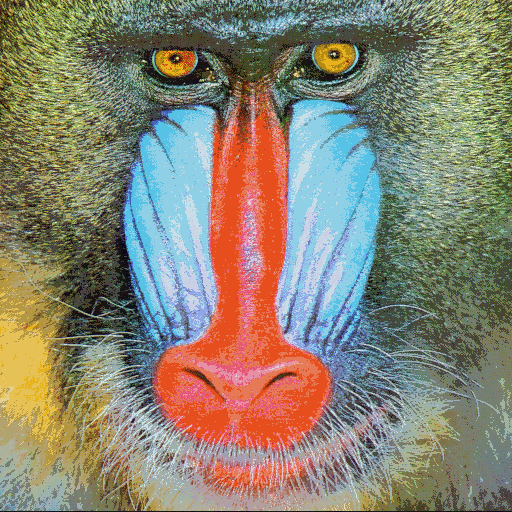
\includegraphics[width=\ww\linewidth]{../zad2/hsv1/I1_444.png }} \hfill%
    \caption{tekst to zmiany} 
    \label{fig:porownanie1} %label który można wykorzystać w tekście za pomocą polecenia \ref{fig:porownanie1}
\end{figure}

\begin{figure}[H]
    \captionsetup[subfloat]{justification=raggedright,singlelinecheck=false, position=bottom,labelformat=empty} %
    \subfloat[----!zad2/hsv2/data:1!----]{\includegraphics[width=\ww\linewidth]{../zad2/hsv2/I1_ori.png }} \hfill%	
    \subfloat[----!zad2/hsv2/data:2!----]{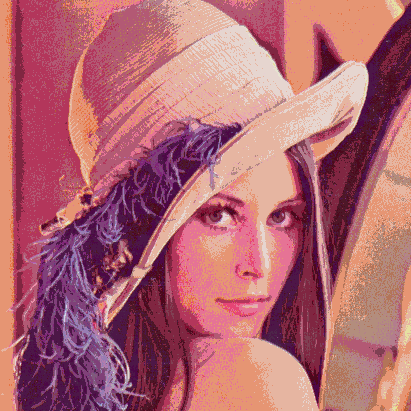
\includegraphics[width=\ww\linewidth]{../zad2/hsv2/I1_222.png }} \hfill%	
    \subfloat[----!zad2/hsv2/data:3!----]{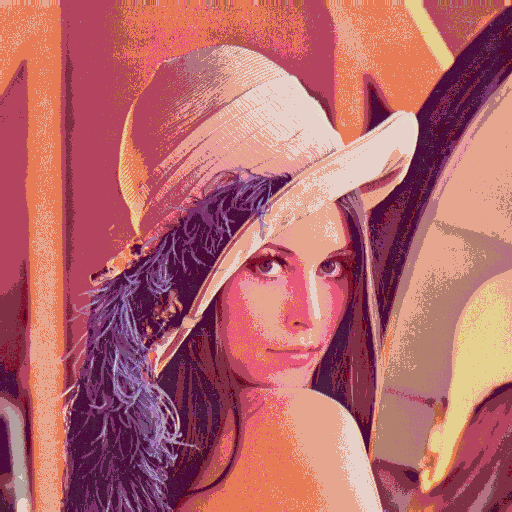
\includegraphics[width=\ww\linewidth]{../zad2/hsv2/I1_444.png }} \hfill%
    \caption{tekst to zmiany} 
    \label{fig:porownanie1} %label który można wykorzystać w tekście za pomocą polecenia \ref{fig:porownanie1}
\end{figure}

\begin{figure}[H]
    \captionsetup[subfloat]{justification=raggedright,singlelinecheck=false, position=bottom,labelformat=empty} %
    \subfloat[----!zad2/hsv3/data:1!----]{\includegraphics[width=\ww\linewidth]{../zad2/hsv3/I1_ori.png }} \hfill%	
    \subfloat[----!zad2/hsv3/data:2!----]{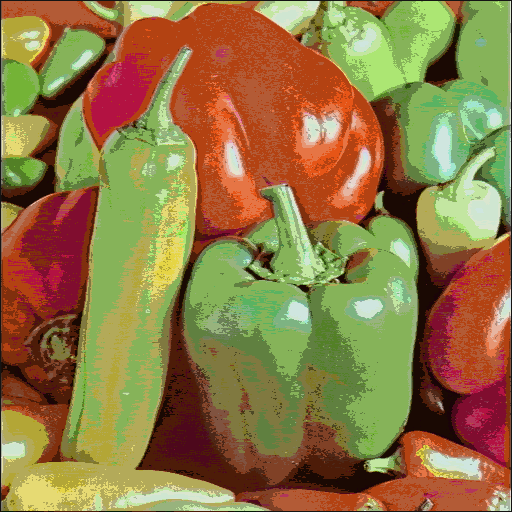
\includegraphics[width=\ww\linewidth]{../zad2/hsv3/I1_222.png }} \hfill%	
    \subfloat[----!zad2/hsv3/data:3!----]{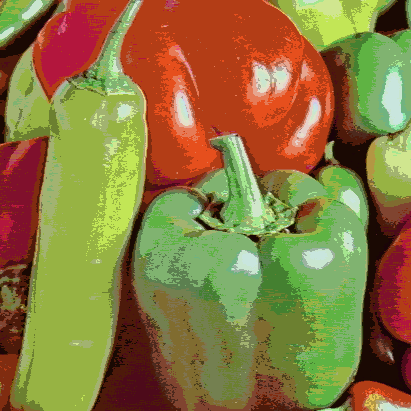
\includegraphics[width=\ww\linewidth]{../zad2/hsv3/I1_444.png }} \hfill%
    \caption{tekst to zmiany} 
    \label{fig:porownanie1} %label który można wykorzystać w tekście za pomocą polecenia \ref{fig:porownanie1}
\end{figure}

\begin{figure}[H]
    \captionsetup[subfloat]{justification=raggedright,singlelinecheck=false, position=bottom,labelformat=empty} %
    \subfloat[----!zad2/hsv4/data:1!----]{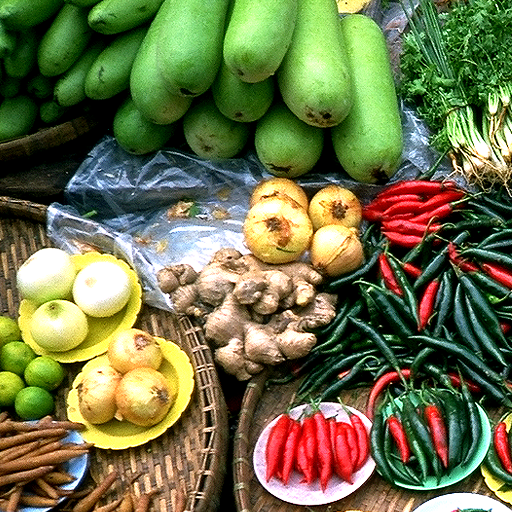
\includegraphics[width=\ww\linewidth]{../zad2/hsv4/I1_ori.png }} \hfill%	
    \subfloat[----!zad2/hsv4/data:2!----]{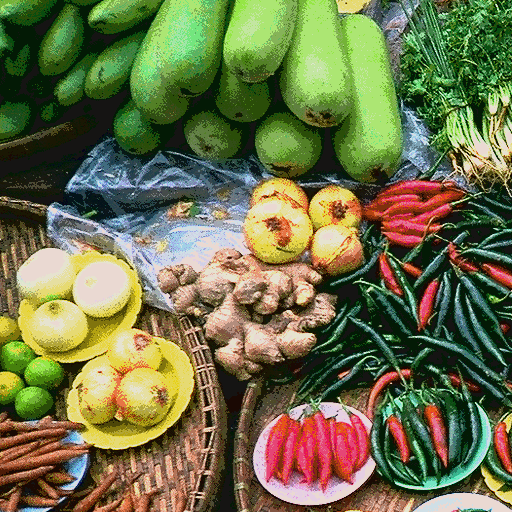
\includegraphics[width=\ww\linewidth]{../zad2/hsv4/I1_222.png }} \hfill%	
    \subfloat[----!zad2/hsv4/data:3!----]{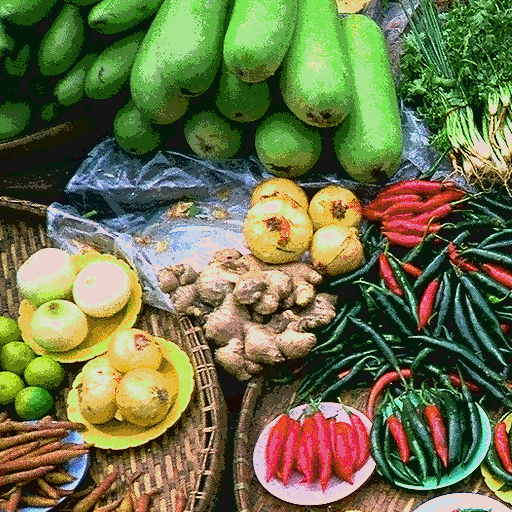
\includegraphics[width=\ww\linewidth]{../zad2/hsv4/I1_444.png }} \hfill%
    \caption{tekst to zmiany} 
    \label{fig:porownanie1} %label który można wykorzystać w tekście za pomocą polecenia \ref{fig:porownanie1}
\end{figure}

\begin{figure}[H]
    \captionsetup[subfloat]{justification=raggedright,singlelinecheck=false, position=bottom,labelformat=empty} %
    \subfloat[----!zad2/hsv5/data:1!----]{\includegraphics[width=\ww\linewidth]{../zad2/hsv5/I1_ori.png }} \hfill%	
    \subfloat[----!zad2/hsv5/data:2!----]{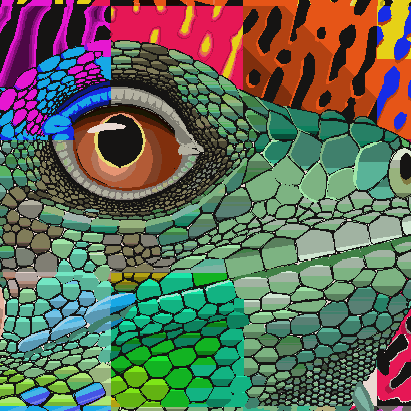
\includegraphics[width=\ww\linewidth]{../zad2/hsv5/I1_222.png }} \hfill%	
    \subfloat[----!zad2/hsv5/data:3!----]{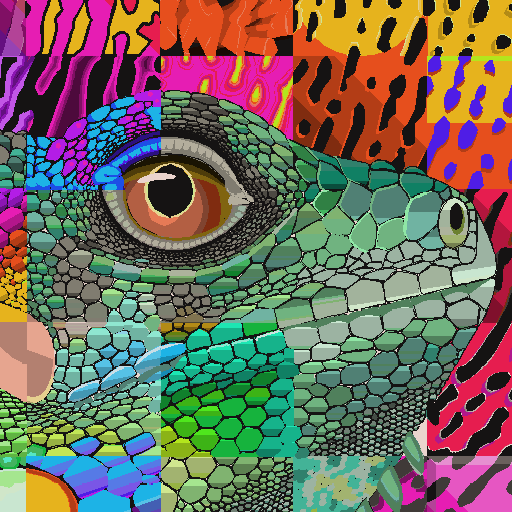
\includegraphics[width=\ww\linewidth]{../zad2/hsv5/I1_444.png }} \hfill%
    \caption{tekst to zmiany} 
    \label{fig:porownanie1} %label który można wykorzystać w tekście za pomocą polecenia \ref{fig:porownanie1}
\end{figure}








\newpage

\section*{Kody Programów}


\definecolor{codegreen}{rgb}{0,0.6,0}
\definecolor{codegray}{rgb}{0.5,0.5,0.5}
\definecolor{codepurple}{rgb}{0.58,0,0.82}
\definecolor{backcolour}{rgb}{0.95,0.95,0.92}

\lstdefinestyle{mystyle}{
    backgroundcolor=\color{backcolour},   
    commentstyle=\color{codegreen},
    keywordstyle=\color{magenta},
    numberstyle=\tiny\color{codegray},
    stringstyle=\color{codepurple},
    basicstyle=\ttfamily\footnotesize,
    breakatwhitespace=false,         
    breaklines=true,                 
    captionpos=b,                    
    keepspaces=true,                 
    numbers=left,                    
    numbersep=5pt,                  
    showspaces=false,                
    showstringspaces=false,
    showtabs=false,                  
    tabsize=2
}


\lstset{style=mystyle}

\subsection*{count\_rgb4.m           } \lstinputlisting[language=Octave]{../matlab/count\_rgb4.m         } \newpage
\subsection*{image\_quantization.m   } \lstinputlisting[language=Octave]{../matlab/image\_quantization.m  } \newpage

 





\end{document}